\newpage
\section{리눅스 커널에 적용}
\label{sec:linux}

%$$$$$$$$$$$$$$$$$$$$$$$$$$$$$$$$$$$$$$$$$$$$$$$$$$$$$$$$$$$$$$$$$$$$$$$$$$$$$$$$
%Paragraph 1: Linux의 reverse mapping에 대한 자세한 설명 
%$$$$$$$$$$$$$$$$$$$$$$$$$$$$$$$$$$$$$$$$$$$$$$$$$$$$$$$$$$$$$$$$$$$$$$$$$$$$$$$$
이번 장은 리눅스 커널의 업데이트 직렬화에 대한 문제를 풀기 위해,
어떻게 LDU를 리눅스 가상 메모리 시스템에 적용했는지에 대해 설명한다.
이러한 리눅스 커널의 가상 메모리 시스템은 리눅스 커널에서 가장 복잡한 부분이며, 
본 장에서는 이처럼 복잡한 가상 메모리 시스템과 보다 구현적인 내용을 다룬다.

리눅스 역 매핑(RMAP)은 커널 메모리 관리 메커니즘(Mechanism) 중 하나 이다.
이것은 익명 역 매핑과 파일 역 매핑으로 구성되며 이것은 업데이트 비율이 높은 자료구조이다.
이러한 두 가지 RMAP은 리눅스의 가상 주소(VMAs)들을 관리하고, 이것은 나중에 물지 주소(Physical Address)를 
가상 주소로 변환할 때 사용된다.
RMAP은 프로세스 간 공유하는 전역 자원(Global Resource)이다.
이러한 전역 자원인 RMAP은 인터벌 트리(Interval Tree)에 의해 관리된다.
이러한 공유 자원을 보호하기 위해, 리눅스는 읽기-쓰기 세마포어(Reader-Writer Semaphore)를 이용하고 있다.
이러한 이유로 결국 동시적으로 많은 프로세스가 생성되면 읽기-쓰기 세마포에 때문에 병목 현상이 된다.
그 이유는 RMAP의 업데이트 연산들은 병렬로 실행되지 못한다. 
뿐만 아니라 락 자체가 캐시 커뮤니케이션 오버헤드를 가져오기 때문이다.

이와 반대로, RMAP은 물리 페이지(Physical Page)가 디스크로 옮겨 질 때, 다른 CPU로 옮겨질 때, 그리고 
파일 사이즈를 줄일 때 간혈적으로 읽는다. 즉 RMAP은 Update-heavy 자료구조이다.

\subsection{익명 역 매핑}


%$$$$$$$$$$$$$$$$$$$$$$$$$$$$$$$$$$$$$$$$$$$$$$$$$$$$$$$$$$$$$$$$$$$$$$$$$$$$$$$$
%Paragraph 1: linux의 anon vma의 공유된 구조에 대한 설명
%$$$$$$$$$$$$$$$$$$$$$$$$$$$$$$$$$$$$$$$$$$$$$$$$$$$$$$$$$$$$$$$$$$$$$$$$$$$$$$$$
그림~\ref{fig:anonvmaramp}은 익명 RMAP에 대한 자료구조를 보여준다.
프로세스가 자식을 만들 때, 부모의 익명 메모리 체인(AVC)는 자식에게 복사한다. 
그리고 새로운 익명 가상메모리(\code{struct anon\_vma})는 생성이 된다.
프로세스가 동시적으로 자식 프로세스를 만들 때, 더 복잡한 익명 RMAP의 자료구조는 생성된다.
또한 익명 RMAP은 리눅스 커널에서 복잡한 자료구조 중 하나이다~\cite{CorbetLWNANON}.
익명 RMAP은 자식 프로세스간 AVCs를 공유하기 때문에 루트(root)의 락을 사용한다.
따라서 이러한 루트 락은 락 경합 문제를 일으킨다~\cite{Andi2011adding}.  

\begin{figure}[tb]
  \begin{center}
     \includegraphics[width=1\textwidth,height=1\textheight,keepaspectratio]{fig/anon_vma}
  \end{center}
  \caption{리눅스 익명 역 매핑에 LDU를 적용한 그림.}
  \label{fig:anonvmaramp}
\end{figure}

%$$$$$$$$$$$$$$$$$$$$$$$$$$$$$$$$$$$$$$$$$$$$$$$$$$$$$$$$$$$$$$$$$$$$$$$$$$$$$$$$
%Paragraph 2: anon vma에 ldu 적용한 방법에 대한 설명 
%$$$$$$$$$$$$$$$$$$$$$$$$$$$$$$$$$$$$$$$$$$$$$$$$$$$$$$$$$$$$$$$$$$$$$$$$$$$$$$$$
락 경합에 대한 문제점을 제거하기 위해서, 우리는 개별적인 오브젝트(\code{struct anon\_vma})에 
삽입과 삭제에 대한 마크 필드를 추가하였다. 
그리고 우리는 업데이트 순간 로그를 지우는 기술을 구현하였다.

또한 로그 큐 헤더에 대한 위치를 이해하는것은 중요하다.
앞에서 설명한봐와 같이, 익명 RMAP은 루트의 락을 사용하기 때문에, 퍼코어 큐 버전의 LDU는 
퍼코어 메모리에 루트의 정보와 함께 저장하거나, 전역 큐의 경우에는 루트 자료구조인 \code{struct anon\_vma}에 
저장한다. 
이와 같이 LDU는 복잡하지 않는 동기화 기법이기 때문에 프로그래머의 노력이 많이 필요하지 않는다.
따라서 원본 자료구조를 많이 수정하지 않는다. 

\subsection{파일 역 매핑}

\begin{figure}[tb]
  \begin{center}
     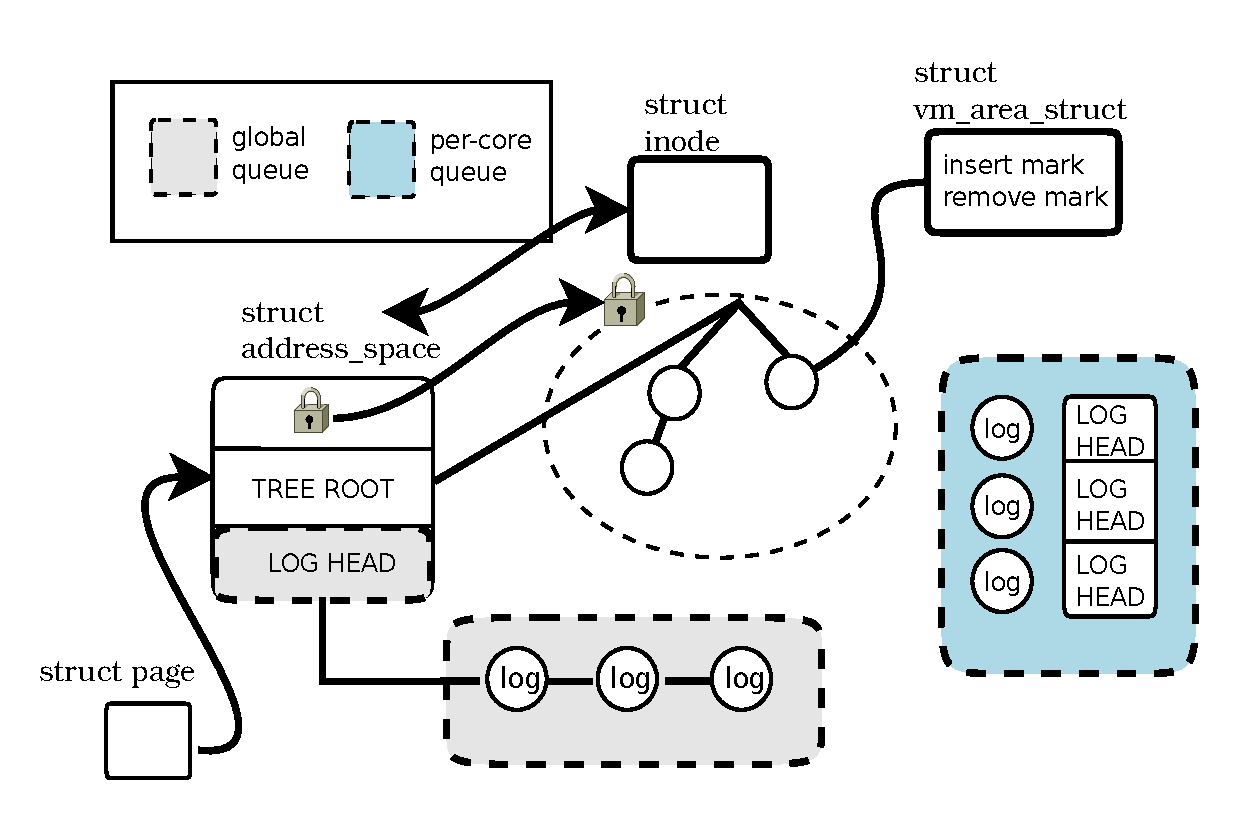
\includegraphics[width=1\textwidth,height=1\textheight,keepaspectratio]{fig/file_rmap}
  \end{center}
  \caption{리눅스 파일 역 매핑에 LDU를 적용한 그림.}
  \label{fig:fileramp}
\end{figure}

%$$$$$$$$$$$$$$$$$$$$$$$$$$$$$$$$$$$$$$$$$$$$$$$$$$$$$$$$$$$$$$$$$$$$$$$$$$$$$$$$
%Paragraph 1: linux의 file mapped page reverse mapping의 구조에 대한 설명
%$$$$$$$$$$$$$$$$$$$$$$$$$$$$$$$$$$$$$$$$$$$$$$$$$$$$$$$$$$$$$$$$$$$$$$$$$$$$$$$$
그림~\ref{fig:fileramp}는 파일에 대한 RMAP을 보여준다.
물리적 주소를 가상 주소로 변경하기 위해서, 페이지는 Address Space 오브젝트(\code{struct address\_space})
를 가리키며, Address Space 오브젝트는 인터벌 트리를 이용하여 VMAs를 관리한다.
이러한 인터벌 트리는 프로세스간 공유하는 자원이다. 
\code{fork()} 그리고 \code{exit()}과 같은 시스템 콜은 VMAs에 대해서 동시적 업데이트를 
수반하므로, 프로세스들이 동시에 많은 시스템 콜을 호출할 때, 
파일 RMAP은 업데이트 연산 때문에 결국 직렬화가 된다. 

%$$$$$$$$$$$$$$$$$$$$$$$$$$$$$$$$$$$$$$$$$$$$$$$$$$$$$$$$$$$$$$$$$$$$$$$$$$$$$$$$
%Paragraph 2: file mapping에 ldu 적용한 방법에 대한 설명 
%$$$$$$$$$$$$$$$$$$$$$$$$$$$$$$$$$$$$$$$$$$$$$$$$$$$$$$$$$$$$$$$$$$$$$$$$$$$$$$$$
LDU는 파일 RMAP 자료구조에 쉽게 적용될 수 있다. 
예를 들어, LDU를 사용하기 위해서는 개발자는 로그 큐 헤더를 퍼코어 메모리에 저장하거나 
아니면 원본 자료구조(\code{struct address\_space})에 저장하면 된다.
그리고 각각의 오브젝트(\code{struct vm\_area\_struct})에 마크필드를 추가하면 된다. 
그리고 개발자는 락 없이 업데이트 함수를 로깅 함수로 수정한다.  
마지막으로 개발자는 \code{synchronize} 함수를 만들고, 이것을 읽기 연산 전에 호출되도록 수정한다.

또한 그림~\ref{fig:fileramp}은 LDU가 추가적으로 전역 큐를 사용하는지를 보여준다. 
이것은 로그의 헤드 포인터가 인터벌 트리의 자료구조에 위치하기 때문이다.
반면에, 퍼코어 큐는 헤드에 대한 메모리의 위치가 다르므로, 추가적인 퍼코어 큐에 대한 관리 방법이 필요하다. 

\subsection{자세한 구현 내용}
%$$$$$$$$$$$$$$$$$$$$$$$$$$$$$$$$$$$$$$$$$$$$$$$$$$$$$$$$$$$$$$$$$$$$$$$$$$$$$$$$
%Paragraph 2: per-core queue 구현에 대한 설명 
%$$$$$$$$$$$$$$$$$$$$$$$$$$$$$$$$$$$$$$$$$$$$$$$$$$$$$$$$$$$$$$$$$$$$$$$$$$$$$$$$L
LDU의 퍼코어 큐는 로그의 헤드 포인트 위치가 큐는 원본 자료구조와 분리 되어 있다.
따라서 퍼코어 큐의 구현은 퍼코어 해시 테이블을 이용하였다. 
이것은 각각의 오브젝트들을 구분 할 수 있게 해준다.
퍼코어 해쉬 테이블은 직접 사상 캐시(Direct-mapped Cache)를 방법으로 구현하였다. 
이것은 하나의 해시 버켓(Bucket)에는 오직 하나의 오브젝트만 존재하는 방법이다.
그 이유는 최근에 사용된 오브젝트가 다시 사용될 확률이 크기 때문이다. 
만약 해쉬 테이블이 충돌을 만나면, LDU는 충돌난 오브젝트를 해쉬 슬롯에서 부터 내보낸다.
더욱이, 이러한 방법은 프로그래머의 추가적인 작업을 줄인다. 
그 이유는 이것은 코드의 수정을 최소화할 수 있고 추가적인 락이 필요가 없기 때문이다.
하지만 퍼코어 해시 테이블은 해시 충돌에 따른 오버헤드를 야기한다.
이러한 방법은 파일 RMAP(\code{struct address\_space})과 같이 적은 빈도수로 루트 
오브젝트가 생성될 때 효율적이다. 
반면에, 익명 RMAP은 극심하게 루트 오브젝트((\code{struct anon\_vma})들을 생성하기 때문에, 
이것은 심한 해쉬 충돌 오버헤드를 발생한다. 
그러므로, 익명 RMAP과 같은 경우에는 오브젝트의 헤더를 구별하지 않았다. 
그러나 이것은 추가적인 프로그래머의 작업과 전역 락이 필요하다.

\begin{figure}[h!]
\begin{center}
\inputminted[linenos,fontsize=\footnotesize,
tabsize=4]{c}{src/ldu_queue_per_core.c}
\end{center}
%\rule{\columnwidth}{0.5pt}
%\vspace{-\baselineskip}
\caption{LDU의 퍼코어 큐.}
\label{fig:glduphysicalupdate}
\end{figure}

%$$$$$$$$$$$$$$$$$$$$$$$$$$$$$$$$$$$$$$$$$$$$$$$$$$$$$$$$$$$$$$$$$$$$$$$$$$$$$$$$
%Paragraph 1: 커널 버전 및 코드 분량, 테스트에 대한 설명
%$$$$$$$$$$$$$$$$$$$$$$$$$$$$$$$$$$$$$$$$$$$$$$$$$$$$$$$$$$$$$$$$$$$$$$$$$$$$$$$$
우리는 새로운 지연 업데이트 알고르즘을 리눅스 4.5-rc6 커널에 구현하였고, 우리의 
수정된 리눅스는 오픈소스로 이용할 수 있다.  
우리의 구현은 충분히 안정적이며, 리눅스의 테스트 
프로젝트(Linux Test Project)~\cite{LTP} 중에서 가상 메모리, 스케줄러 그리고 
파일과 관련된 테스트를 모두 통과하였다. 
수정된 소스 코드의 라인 수는 LDU의 전역 큐 버전은 564라인을 수정하였고, 
LDU의 퍼코어 큐 버전은 807라인을 수정하였다. 
그 이유는 퍼코어 버전이 전역 큐 버전에 비해 복잡하다는 것을 의미한다.


